\section{Distributed Formation Control Strategy} \label{sec:0control}
The formation control strategy aims to form, maintain and self-reconfigurate the V-shape formation in response to obstacles and narrow passages during UAV navigation. This adaptation is achieved through either expanding/shrinking two wings of the V-shape. It allows the UAV formation to navigate safely within confined spaces without encountering collisions. The proposed algorithm operates based on the use of distributed behavior-based control and artificial potential field approaches so that individual UAVs can make decisions and adjust the formation shape as needed. The strategy consists of two parts: maintaining formation and reconfigurating formation.

\begin{figure*}
    \centering
    \begin{subfigure}[b]{0.32\textwidth}
    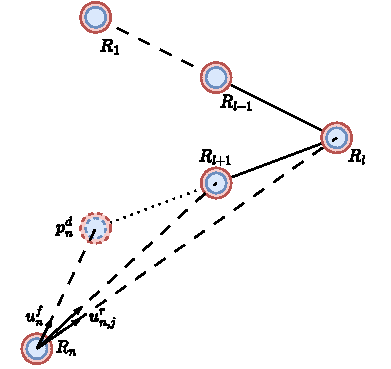
\includegraphics[width=\textwidth]{paper1/images/reconfiguration0.pdf}
    \caption{Disruption in formation}
    \label{fig:chap2_reconfig0}
    \end{subfigure}
    \begin{subfigure}[b]{0.32\textwidth}
    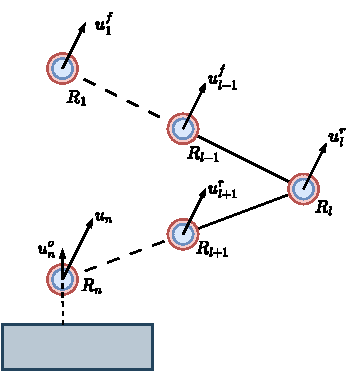
\includegraphics[width=\textwidth]{paper1/images/reconfiguration1.pdf}
    \caption{Obstacles from one side}
    \label{fig:chap2_reconfig1}
    \end{subfigure}
    \begin{subfigure}[b]{0.32\textwidth}
    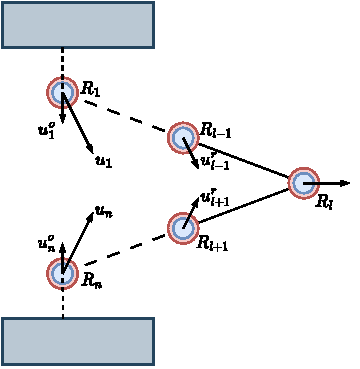
\includegraphics[width=\textwidth]{paper1/images/reconfiguration2.pdf}
    \caption{Obstacles from both sides}
    \label{fig:chap2_reconfig2}
    \end{subfigure}
    \caption{Self-reconfiguration of the V-shape formation based on the mechanism of pliers or scissors}
    \label{fig:chap2_reconfiguration}
\end{figure*}

\subsection{Formation maintenance strategy}
Behavior-based control is the approach that combines a set of distributed control modules, called behaviors, to achieve the desired objective \cite{Mataric2008, 736776}. In this work, the UAV formation is maintained based on the combination of the following behaviors.
\subsubsection{Formation behavior}
The formation behavior aims to guide UAVs to achieve their desired positions within the predefined formation. According to \eqref{eqn:chap2_desired_pose}, the desired position $p_i^d$ of UAV $R_i$ in the formation can be obtained. Inspired by \cite{Dang2019,MirzaeeKahagh2020}, we define the formation behavior as follows:
\begin{equation}
    u_i^f=-k_f\left(p_i- p_i^d\right) + u_l,
    \label{eqn:chap2_uf}
\end{equation}
where $k_f>0$ is a positive formation gain. 

\subsubsection{Goal reaching behavior}
This behavior navigates the formation towards the desired location. To accomplish this objective, a target-tracking controller is formulated based on the relative position between the leader UAV and the goal. Let $p_g$ be the goal position that the formation needs to reach. The goal reaching behavior is constructed as follows: 
\begin{equation}
    u_i^g=-k_g\left(p_i - p_g\right),
    \label{eqn:chap2_ug}
\end{equation}
where $k_g>0$ is a positive tracking gain.

\subsubsection{Obstacle avoidance behavior}
During operation, the formation must avoid obstacles present in the environment. Let $p_{io_h}$ be the closest point on the boundary of obstacle $o_h$ within the sensing range of UAV $R_i$. When that UAV senses obstacle $o_h$, it will create a thrust to maneuver and avoid the obstacle. The thrust is directed as follows:
\begin{equation}
    u_{ih}^{o}=\left\{ \begin{array}{cc}
-k_o\left(\dfrac{1}{d_{io_h}^2} - \dfrac{1}{r_s^2}\right)\dfrac{p_i-p_{io_h}}{\left\Vert p_i-p_{io_h}\right\Vert}, & \text{if } d_{io_h} < r_s\\
0. & \text{otherwise}\\
\end{array}\right.
\end{equation}
where $k_o>0$ is a positive gain; $d_{io_h}$ is the distance between UAV $R_i$ and obstacle $o_h$. When considering all obstacles, the obstacle avoidance behavior of UAV $R_i$ are obtained as follows:
\begin{equation}
    u_i^o=\sum_{h=1}^m{u_{ih}},
    \label{eqn:chap2_uo}
\end{equation}
where $m$ is number of observable obstacles within the sensing range of UAV $R_i$.

\subsubsection{Collision avoidance behavior}
Apart from avoiding obstacles, the control algorithm also needs to adjust the UAV positions to avoid collision among them. To address this, we propose that UAVs $R_i$ and $R_j$ that are not in the same wing but within each other's sensing area, i.e., $\left\Vert p_{ij}\right\Vert < r_{s}$, will exert a repulsive force to preventing the UAVs from entering the alert area $S_a$. Let $p_{ij}=p_i-p_j$. The collision avoidance behavior is determined as follows:
\begin{equation}
    u_{ij}^{c}=k_{c}\dfrac{e^{-\beta_{c}\left(\left\Vert p_{ij}\right\Vert -r_{a}\right)}}{\left\Vert p_{ij}\right\Vert -r_{a}}\dfrac{p_i-p_j}{\left\Vert p_i-p_j\right\Vert},
    \label{eqn:chap2_uc}
\end{equation}
where $k_c>0$ is a positive collision gain.

%The collision avoidance behavior of UAV in the same wing is further introduced in Section \ref{sec:0reconfig}.

\subsection{Self-reconfigurable formation strategy} 
\label{sec:0reconfig}
\begin{figure*}
    \centering
    \begin{subfigure}[b]{\textwidth}
        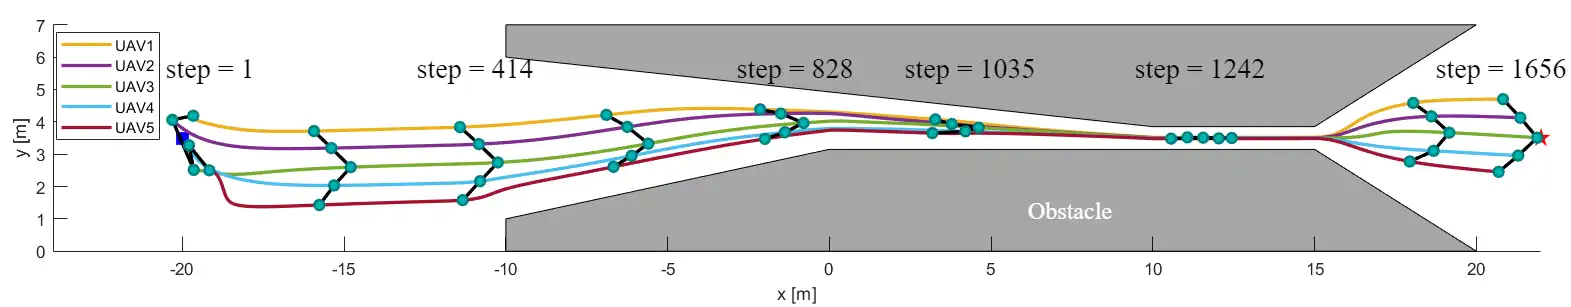
\includegraphics[width=\textwidth]{paper1/images/result.png}
        \caption{Trajectories of the UAVs in the formation}
        \label{fig:chap2_motion}
    \end{subfigure}
    \begin{subfigure}[b]{\textwidth}
        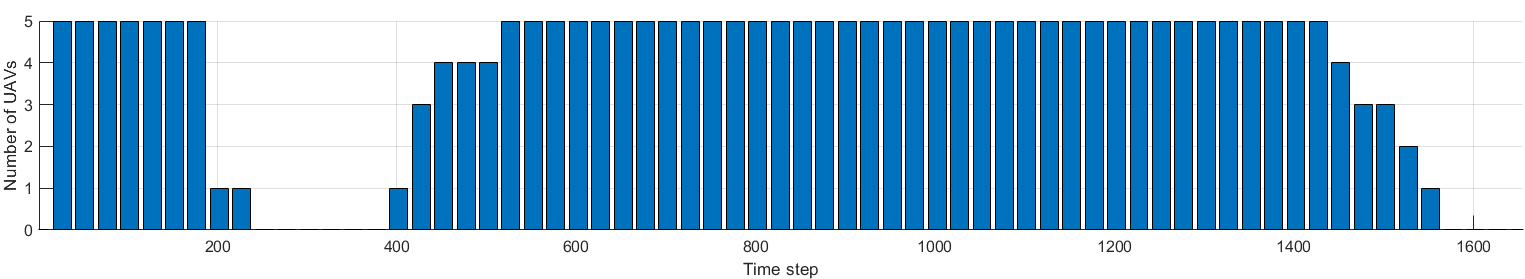
\includegraphics[width=\textwidth]{paper1/images/number.png}
        \caption{Number of UAVs activating reconfiguration behaviors over time}
        \label{fig:chap2_number}
    \end{subfigure}
    \caption{Simulation result of the V-shape formation moving through a narrow passage}
    \label{fig:chap2_result}
\end{figure*}

Inspired by the mechanics of pliers and scissors, which alter their shape through the application of opposing forces on their handle arms, the V-shape formation can open or close its wings based on the exertion of external forces. In our work, the force is produced based on the difference in the distances among the UAVs and their desired distances. Specifically, in case the formation encounters disruptions arising from improper positioning, as illustrated in Figure \ref{fig:chap2_reconfig0} where UAV $R_n$ deviates from the alignment, the combined force acts to guide it toward its desired location.

In the scenario depicted by Figure \ref{fig:chap2_reconfig1} where a force is exerted from one side, UAV $R_n$ responds by generating a thrust $u_n^o$ to avoid a potential collision with obstacles thus resulting in the control signal $u_n$. Accordingly, other UAVs on the same V-wing, including the leader UAV, also adjust their position based on the behavior control signal $u_i^r$. As the leader UAV $R_l$ changes its position, the UAVs on the opposing wing realign themselves by formation behavior $u_i^f$. As a result, the whole UAV formation tends to move towards the other side.

In another scenario, when obstacles impact the formation from both opposing sides, as depicted in Figure \ref{fig:chap2_reconfig2}, they affect UAVs $R_1$ and $R_n$, leading to the generation of obstacle avoidance behaviors denoted as $u_1^o$ and $u_n^o$. Other UAVs on the same wing respond by generating reconfiguration behaviors $u_i^r$ that adjust the UAVs' position accordingly. As a result, the V-shape formation is able to shrink its wing to travel through narrow passages.

In our work, the aforementioned reconfiguration idea is implemented by the following equation:

\begin{equation}
    u_{ij}^{r}=k_{r}\dfrac{\left|\left\Vert p_{ij}\right\Vert -d_{ij}\right|^{\beta_r}}{\left(\left\Vert p_{ij}\right\Vert -r_{a}\right)^{2}}\dfrac{p_i-p_j}{\left\Vert p_i-p_j\right\Vert},
    \label{eqn:chap2_ur}
\end{equation}
where $k_r>0$ is a positive reconfiguration gain, $\beta_r>0$ is the smoothness factor, $d_{ij}$ is the desired distance between two UAVs $R_i$ and $R_j$ n the same wing, $d_{ij}=d\left\vert i-j\right\vert$. In (\ref{eqn:chap2_ur}), the term $\left|\left\Vert p_{ij}\right\Vert -d_{ij}\right|$ enables the UAVs to adjust their positions so that the desired distances among the UAVs are maintained. This behavior is also used as a collision avoidance behavior for the UAVs in the same wing.

\subsection{Overall strategy}
The overall distributed control strategy is obtained by combining the behaviors from all UAVs as follows:%, from operating to control parameters, which formulated as follows:
\begin{equation}
    u_{i}=\left\{ \begin{array}{cc}
u_{i}^{g}+u_{i}^{r}+u_{i}^{c}+u_{i}^{o}, & \text{if assigned as leader}\\
u_{i}^{f}+u_{i}^{r}+u_{i}^{c}+u_{i}^{o}. & \text{otherwise}
\end{array}\right.
\end{equation}

According to this function, the behaviors are automatically triggered in response to external influences or disturbances encountered by the formation. Once the desired state is achieved, the behavioral values are maintained resulting in stable operation of the UAV formation.